\documentclass[1p]{elsarticle_modified}
%\bibliographystyle{elsarticle-num}

%\usepackage[colorlinks]{hyperref}
%\usepackage{abbrmath_seonhwa} %\Abb, \Ascr, \Acal ,\Abf, \Afrak
\usepackage{amsfonts}
\usepackage{amssymb}
\usepackage{amsmath}
\usepackage{amsthm}
\usepackage{scalefnt}
\usepackage{amsbsy}
\usepackage{kotex}
\usepackage{caption}
\usepackage{subfig}
\usepackage{color}
\usepackage{graphicx}
\usepackage{xcolor} %% white, black, red, green, blue, cyan, magenta, yellow
\usepackage{float}
\usepackage{setspace}
\usepackage{hyperref}

\usepackage{tikz}
\usetikzlibrary{arrows}

\usepackage{multirow}
\usepackage{array} % fixed length table
\usepackage{hhline}

%%%%%%%%%%%%%%%%%%%%%
\makeatletter
\renewcommand*\env@matrix[1][\arraystretch]{%
	\edef\arraystretch{#1}%
	\hskip -\arraycolsep
	\let\@ifnextchar\new@ifnextchar
	\array{*\c@MaxMatrixCols c}}
\makeatother %https://tex.stackexchange.com/questions/14071/how-can-i-increase-the-line-spacing-in-a-matrix
%%%%%%%%%%%%%%%

\usepackage[normalem]{ulem}

\newcommand{\msout}[1]{\ifmmode\text{\sout{\ensuremath{#1}}}\else\sout{#1}\fi}
%SOURCE: \msout is \stkout macro in https://tex.stackexchange.com/questions/20609/strikeout-in-math-mode

\newcommand{\cancel}[1]{
	\ifmmode
	{\color{red}\msout{#1}}
	\else
	{\color{red}\sout{#1}}
	\fi
}

\newcommand{\add}[1]{
	{\color{blue}\uwave{#1}}
}

\newcommand{\replace}[2]{
	\ifmmode
	{\color{red}\msout{#1}}{\color{blue}\uwave{#2}}
	\else
	{\color{red}\sout{#1}}{\color{blue}\uwave{#2}}
	\fi
}

\newcommand{\Sol}{\mathcal{S}} %segment
\newcommand{\D}{D} %diagram
\newcommand{\A}{\mathcal{A}} %arc


%%%%%%%%%%%%%%%%%%%%%%%%%%%%%5 test

\def\sl{\operatorname{\textup{SL}}(2,\Cbb)}
\def\psl{\operatorname{\textup{PSL}}(2,\Cbb)}
\def\quan{\mkern 1mu \triangleright \mkern 1mu}

\theoremstyle{definition}
\newtheorem{thm}{Theorem}[section]
\newtheorem{prop}[thm]{Proposition}
\newtheorem{lem}[thm]{Lemma}
\newtheorem{ques}[thm]{Question}
\newtheorem{cor}[thm]{Corollary}
\newtheorem{defn}[thm]{Definition}
\newtheorem{exam}[thm]{Example}
\newtheorem{rmk}[thm]{Remark}
\newtheorem{alg}[thm]{Algorithm}

\newcommand{\I}{\sqrt{-1}}
\begin{document}

%\begin{frontmatter}
%
%\title{Boundary parabolic representations of knots up to 8 crossings}
%
%%% Group authors per affiliation:
%\author{Yunhi Cho} 
%\address{Department of Mathematics, University of Seoul, Seoul, Korea}
%\ead{yhcho@uos.ac.kr}
%
%
%\author{Seonhwa Kim} %\fnref{s_kim}}
%\address{Center for Geometry and Physics, Institute for Basic Science, Pohang, 37673, Korea}
%\ead{ryeona17@ibs.re.kr}
%
%\author{Hyuk Kim}
%\address{Department of Mathematical Sciences, Seoul National University, Seoul 08826, Korea}
%\ead{hyukkim@snu.ac.kr}
%
%\author{Seokbeom Yoon}
%\address{Department of Mathematical Sciences, Seoul National University, Seoul, 08826,  Korea}
%\ead{sbyoon15@snu.ac.kr}
%
%\begin{abstract}
%We find all boundary parabolic representation of knots up to 8 crossings.
%
%\end{abstract}
%\begin{keyword}
%    \MSC[2010] 57M25 
%\end{keyword}
%
%\end{frontmatter}

%\linenumbers
%\tableofcontents
%
\newcommand\colored[1]{\textcolor{white}{\rule[-0.35ex]{0.8em}{1.4ex}}\kern-0.8em\color{red} #1}%
%\newcommand\colored[1]{\textcolor{white}{ #1}\kern-2.17ex	\textcolor{white}{ #1}\kern-1.81ex	\textcolor{white}{ #1}\kern-2.15ex\color{red}#1	}

{\Large $\underline{12n_{0059}~(K12n_{0059})}$}

\setlength{\tabcolsep}{10pt}
\renewcommand{\arraystretch}{1.6}
\vspace{1cm}\begin{tabular}{m{100pt}>{\centering\arraybackslash}m{274pt}}
\multirow{5}{120pt}{
	\centering
	\includegraphics[width=112pt]{../../../GIT/diagram.site/Diagrams/png/2148_12n_0059.png}\\
\ \ \ A knot diagram\footnotemark}&
\allowdisplaybreaks
\textbf{Linearized knot diagam} \\
\cline{2-2}
 &
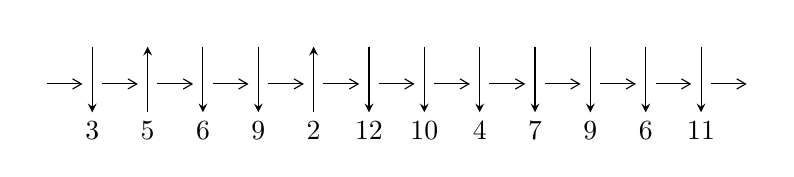
\begin{tikzpicture}[x=20pt, y=17pt]
	% nodes
	\node (C0) at (0, 0) {};
	\node (C1) at (1, 0) {};
	\node (C1U) at (1, +1) {};
	\node (C1D) at (1, -1) {3};

	\node (C2) at (2, 0) {};
	\node (C2U) at (2, +1) {};
	\node (C2D) at (2, -1) {5};

	\node (C3) at (3, 0) {};
	\node (C3U) at (3, +1) {};
	\node (C3D) at (3, -1) {6};

	\node (C4) at (4, 0) {};
	\node (C4U) at (4, +1) {};
	\node (C4D) at (4, -1) {9};

	\node (C5) at (5, 0) {};
	\node (C5U) at (5, +1) {};
	\node (C5D) at (5, -1) {2};

	\node (C6) at (6, 0) {};
	\node (C6U) at (6, +1) {};
	\node (C6D) at (6, -1) {12};

	\node (C7) at (7, 0) {};
	\node (C7U) at (7, +1) {};
	\node (C7D) at (7, -1) {10};

	\node (C8) at (8, 0) {};
	\node (C8U) at (8, +1) {};
	\node (C8D) at (8, -1) {4};

	\node (C9) at (9, 0) {};
	\node (C9U) at (9, +1) {};
	\node (C9D) at (9, -1) {7};

	\node (C10) at (10, 0) {};
	\node (C10U) at (10, +1) {};
	\node (C10D) at (10, -1) {9};

	\node (C11) at (11, 0) {};
	\node (C11U) at (11, +1) {};
	\node (C11D) at (11, -1) {6};

	\node (C12) at (12, 0) {};
	\node (C12U) at (12, +1) {};
	\node (C12D) at (12, -1) {11};
	\node (C13) at (13, 0) {};

	% arrows
	\draw[->,>={angle 60}]
	(C0) edge (C1) (C1) edge (C2) (C2) edge (C3) (C3) edge (C4) (C4) edge (C5) (C5) edge (C6) (C6) edge (C7) (C7) edge (C8) (C8) edge (C9) (C9) edge (C10) (C10) edge (C11) (C11) edge (C12) (C12) edge (C13) ;	\draw[->,>=stealth]
	(C1U) edge (C1D) (C2D) edge (C2U) (C3U) edge (C3D) (C4U) edge (C4D) (C5D) edge (C5U) (C6U) edge (C6D) (C7U) edge (C7D) (C8U) edge (C8D) (C9U) edge (C9D) (C10U) edge (C10D) (C11U) edge (C11D) (C12U) edge (C12D) ;
	\end{tikzpicture} \\
\hhline{~~} \\& 
\textbf{Solving Sequence} \\ \cline{2-2} 
 &
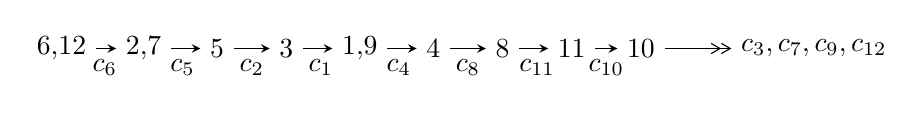
\begin{tikzpicture}[x=25pt, y=7pt]
	% node
	\node (A0) at (-1/8, 0) {6,12};
	\node (A1) at (17/16, 0) {2,7};
	\node (A2) at (17/8, 0) {5};
	\node (A3) at (25/8, 0) {3};
	\node (A4) at (67/16, 0) {1,9};
	\node (A5) at (21/4, 0) {4};
	\node (A6) at (25/4, 0) {8};
	\node (A7) at (29/4, 0) {11};
	\node (A8) at (33/4, 0) {10};
	\node (C1) at (1/2, -1) {$c_{6}$};
	\node (C2) at (13/8, -1) {$c_{5}$};
	\node (C3) at (21/8, -1) {$c_{2}$};
	\node (C4) at (29/8, -1) {$c_{1}$};
	\node (C5) at (19/4, -1) {$c_{4}$};
	\node (C6) at (23/4, -1) {$c_{8}$};
	\node (C7) at (27/4, -1) {$c_{11}$};
	\node (C8) at (31/4, -1) {$c_{10}$};
	\node (A9) at (43/4, 0) {$c_{3},c_{7},c_{9},c_{12}$};

	% edge
	\draw[->,>=stealth]	
	(A0) edge (A1) (A1) edge (A2) (A2) edge (A3) (A3) edge (A4) (A4) edge (A5) (A5) edge (A6) (A6) edge (A7) (A7) edge (A8) ;
	\draw[->>,>={angle 60}]	
	(A8) edge (A9);
\end{tikzpicture} \\ 

\end{tabular} \\

\footnotetext{
The image of knot diagram is generated by the software ``\textbf{Draw programme}" developed by Andrew Bartholomew(\url{http://www.layer8.co.uk/maths/draw/index.htm\#Running-draw}), where we modified some parts for our purpose(\url{https://github.com/CATsTAILs/LinksPainter}).
}\phantom \\ \newline 
\centering \textbf{Ideals for irreducible components\footnotemark of $X_{\text{par}}$} 
 
\begin{align*}
I^u_{1}&=\langle 
- u^{11}+5 u^{10}-14 u^9+25 u^8-36 u^7+34 u^6-22 u^5-2 u^4-3 u^3+u^2+16 d-20 u+1,\\
\phantom{I^u_{1}}&\phantom{= \langle  }- u^{11}+5 u^{10}-14 u^9+25 u^8-36 u^7+34 u^6-22 u^5-2 u^4-3 u^3+u^2+16 c-36 u+1,\\
\phantom{I^u_{1}}&\phantom{= \langle  }-4 u^{12}+19 u^{11}-47 u^{10}+68 u^9-73 u^8+26 u^7+46 u^6-108 u^5+22 u^4+27 u^3-111 u^2+16 b-48 u+7,\\
\phantom{I^u_{1}}&\phantom{= \langle  }-11 u^{12}+51 u^{11}+\cdots+16 a+2,\\
\phantom{I^u_{1}}&\phantom{= \langle  }u^{13}-5 u^{12}+13 u^{11}-20 u^{10}+22 u^9-9 u^8-14 u^7+36 u^6-19 u^5-3 u^4+33 u^3-4 u+1\rangle \\
I^u_{2}&=\langle 
-953 u^9+3087 u^8+\cdots+16432 d+4012,\\
\phantom{I^u_{2}}&\phantom{= \langle  }u^9-3 u^8+5 u^7+3 u^6-12 u^5+10 u^4+17 u^3-18 u^2+16 c-23 u+8,\\
\phantom{I^u_{2}}&\phantom{= \langle  }1173 u^9-2403 u^8+\cdots+32864 b-14956,\;-5403 u^9+34813 u^8+\cdots+131456 a-281772,\\
\phantom{I^u_{2}}&\phantom{= \langle  }u^{10}-3 u^9+5 u^8+3 u^7-12 u^6+10 u^5+17 u^4-18 u^3-23 u^2+8 u+16\rangle \\
I^u_{3}&=\langle 
d-1,\;c-1,\;2 b- a-1,\;a^2+3,\;u-1\rangle \\
I^u_{4}&=\langle 
d,\;c+1,\;b,\;a-1,\;u+1\rangle \\
I^u_{5}&=\langle 
d- c+1,\;2 c b- c a- c- b+a+1,\;a^2 c- b a- a^2+3 c- b-1,\;b^2- b+1,\;u-1\rangle \\
\\
I^v_{1}&=\langle 
a,\;d-1,\;b a+c+b- a,\;b^2- b+1,\;v+1\rangle \\
\end{align*}
\raggedright * 5 irreducible components of $\dim_{\mathbb{C}}=0$, with total 28 representations.\\
\raggedright * 1 irreducible components of $\dim_{\mathbb{C}}=1$ \\
\footnotetext{All coefficients of polynomials are rational numbers. But the coefficients are sometimes approximated in decimal forms when there is not enough margin.}
\newpage
\renewcommand{\arraystretch}{1}
\centering \section*{I. $I^u_{1}= \langle - u^{11}+5 u^{10}+\cdots+16 d+1,\;- u^{11}+5 u^{10}+\cdots+16 c+1,\;-4 u^{12}+19 u^{11}+\cdots+16 b+7,\;-11 u^{12}+51 u^{11}+\cdots+16 a+2,\;u^{13}-5 u^{12}+\cdots-4 u+1 \rangle$}
\flushleft \textbf{(i) Arc colorings}\\
\begin{tabular}{m{7pt} m{180pt} m{7pt} m{180pt} }
\flushright $a_{6}=$&$\begin{pmatrix}1\\0\end{pmatrix}$ \\
\flushright $a_{12}=$&$\begin{pmatrix}0\\u\end{pmatrix}$ \\
\flushright $a_{2}=$&$\begin{pmatrix}0.687500 u^{12}-3.18750 u^{11}+\cdots+8.68750 u-0.125000\\\frac{1}{4} u^{12}-\frac{19}{16} u^{11}+\cdots+3 u-\frac{7}{16}\end{pmatrix}$ \\
\flushright $a_{7}=$&$\begin{pmatrix}1\\u^2\end{pmatrix}$ \\
\flushright $a_{5}=$&$\begin{pmatrix}\frac{9}{8} u^{12}-\frac{87}{16} u^{11}+\cdots+\frac{49}{8} u-\frac{41}{16}\\\frac{5}{16} u^{12}-\frac{3}{2} u^{11}+\cdots+\frac{15}{16} u-\frac{17}{16}\end{pmatrix}$ \\
\flushright $a_{3}=$&$\begin{pmatrix}\frac{9}{8} u^{12}-\frac{85}{16} u^{11}+\cdots+\frac{37}{4} u-\frac{57}{16}\\\frac{3}{16} u^{12}-\frac{7}{8} u^{11}+\cdots+\frac{29}{16} u-\frac{17}{16}\end{pmatrix}$ \\
\flushright $a_{1}=$&$\begin{pmatrix}- u^3\\- u^3+u\end{pmatrix}$ \\
\flushright $a_{9}=$&$\begin{pmatrix}\frac{1}{16} u^{11}-\frac{5}{16} u^{10}+\cdots+\frac{9}{4} u-\frac{1}{16}\\\frac{1}{16} u^{11}-\frac{5}{16} u^{10}+\cdots+\frac{5}{4} u-\frac{1}{16}\end{pmatrix}$ \\
\flushright $a_{4}=$&$\begin{pmatrix}0.937500 u^{12}-4.43750 u^{11}+\cdots+7.43750 u-2.50000\\\frac{3}{16} u^{12}-\frac{7}{8} u^{11}+\cdots+\frac{29}{16} u-\frac{17}{16}\end{pmatrix}$ \\
\flushright $a_{8}=$&$\begin{pmatrix}-\frac{1}{16} u^{12}+\frac{5}{16} u^{11}+\cdots+\frac{1}{16} u-1\\-0.0625000 u^{12}+0.312500 u^{11}+\cdots-2.25000 u^{2}+0.0625000 u\end{pmatrix}$ \\
\flushright $a_{11}=$&$\begin{pmatrix}u\\u\end{pmatrix}$ \\
\flushright $a_{10}=$&$\begin{pmatrix}\frac{1}{16} u^{11}-\frac{5}{16} u^{10}+\cdots+\frac{5}{4} u-\frac{1}{16}\\\frac{1}{16} u^{11}-\frac{5}{16} u^{10}+\cdots+\frac{5}{4} u-\frac{1}{16}\end{pmatrix}$\\&\end{tabular}
\flushleft \textbf{(ii) Obstruction class $= -1$}\\~\\
\flushleft \textbf{(iii) Cusp Shapes $= -\frac{5}{4} u^{12}+\frac{47}{8} u^{11}-\frac{113}{8} u^{10}+\frac{75}{4} u^9-\frac{127}{8} u^8-\frac{19}{4} u^7+\frac{129}{4} u^6-\frac{101}{2} u^5+\frac{31}{2} u^4+\frac{135}{8} u^3-\frac{385}{8} u^2-\frac{9}{4} u-\frac{3}{8}$}\\~\\
\newpage\renewcommand{\arraystretch}{1}
\flushleft \textbf{(iv) u-Polynomials at the component}\newline \\
\begin{tabular}{m{50pt}|m{274pt}}
Crossings & \hspace{64pt}u-Polynomials at each crossing \\
\hline $$\begin{aligned}c_{1}\end{aligned}$$&$\begin{aligned}
&u^{13}+3 u^{12}+\cdots+104 u-16
\end{aligned}$\\
\hline $$\begin{aligned}c_{2},c_{5}\end{aligned}$$&$\begin{aligned}
&u^{13}+u^{12}+\cdots+12 u+4
\end{aligned}$\\
\hline $$\begin{aligned}c_{3}\end{aligned}$$&$\begin{aligned}
&u^{13}- u^{12}+\cdots+1508 u+548
\end{aligned}$\\
\hline $$\begin{aligned}c_{4},c_{8}\end{aligned}$$&$\begin{aligned}
&u^{13}-3 u^{12}+\cdots-32 u+32
\end{aligned}$\\
\hline $$\begin{aligned}c_{6},c_{7},c_{9}\\c_{11}\end{aligned}$$&$\begin{aligned}
&u^{13}-5 u^{12}+\cdots-4 u+1
\end{aligned}$\\
\hline $$\begin{aligned}c_{10},c_{12}\end{aligned}$$&$\begin{aligned}
&u^{13}- u^{12}+\cdots+16 u+1
\end{aligned}$\\
\hline
\end{tabular}\\~\\
\newpage\renewcommand{\arraystretch}{1}
\flushleft \textbf{(v) Riley Polynomials at the component}\newline \\
\begin{tabular}{m{50pt}|m{274pt}}
Crossings & \hspace{64pt}Riley Polynomials at each crossing \\
\hline $$\begin{aligned}c_{1}\end{aligned}$$&$\begin{aligned}
&y^{13}+15 y^{12}+\cdots+21024 y-256
\end{aligned}$\\
\hline $$\begin{aligned}c_{2},c_{5}\end{aligned}$$&$\begin{aligned}
&y^{13}+3 y^{12}+\cdots+104 y-16
\end{aligned}$\\
\hline $$\begin{aligned}c_{3}\end{aligned}$$&$\begin{aligned}
&y^{13}+27 y^{12}+\cdots+1970472 y-300304
\end{aligned}$\\
\hline $$\begin{aligned}c_{4},c_{8}\end{aligned}$$&$\begin{aligned}
&y^{13}+15 y^{12}+\cdots+15616 y^2-1024
\end{aligned}$\\
\hline $$\begin{aligned}c_{6},c_{7},c_{9}\\c_{11}\end{aligned}$$&$\begin{aligned}
&y^{13}+y^{12}+\cdots+16 y-1
\end{aligned}$\\
\hline $$\begin{aligned}c_{10},c_{12}\end{aligned}$$&$\begin{aligned}
&y^{13}+25 y^{12}+\cdots-260 y-1
\end{aligned}$\\
\hline
\end{tabular}\\~\\
\newpage\flushleft \textbf{(vi) Complex Volumes and Cusp Shapes}
$$\begin{array}{c|c|c}  
\text{Solutions to }I^u_{1}& \I (\text{vol} + \sqrt{-1}CS) & \text{Cusp shape}\\
 \hline 
\begin{aligned}
u &= -0.801603 + 0.173700 I \\
a &= \phantom{-}0.33896 - 2.10199 I \\
b &= -0.386403 - 0.917053 I \\
c &= -2.30333 + 2.55112 I \\
d &= -1.50172 + 2.37742 I\end{aligned}
 & -2.92013 + 2.62586 I & -15.8235 - 5.3570 I \\ \hline\begin{aligned}
u &= -0.801603 - 0.173700 I \\
a &= \phantom{-}0.33896 + 2.10199 I \\
b &= -0.386403 + 0.917053 I \\
c &= -2.30333 - 2.55112 I \\
d &= -1.50172 - 2.37742 I\end{aligned}
 & -2.92013 - 2.62586 I & -15.8235 + 5.3570 I \\ \hline\begin{aligned}
u &= \phantom{-}0.536277 + 1.193890 I \\
a &= -0.51569 - 1.90253 I \\
b &= \phantom{-}0.543511 - 1.275200 I \\
c &= -0.123143 + 1.043180 I \\
d &= -0.659420 - 0.150709 I\end{aligned}
 & \phantom{-}1.88235 - 4.50009 I & -8.08386 + 3.64476 I \\ \hline\begin{aligned}
u &= \phantom{-}0.536277 - 1.193890 I \\
a &= -0.51569 + 1.90253 I \\
b &= \phantom{-}0.543511 + 1.275200 I \\
c &= -0.123143 - 1.043180 I \\
d &= -0.659420 + 0.150709 I\end{aligned}
 & \phantom{-}1.88235 + 4.50009 I & -8.08386 - 3.64476 I \\ \hline\begin{aligned}
u &= -0.16802 + 1.50582 I \\
a &= \phantom{-}0.228716 + 0.403848 I \\
b &= \phantom{-}1.124080 + 0.602862 I \\
c &= \phantom{-}0.040508 + 0.923402 I \\
d &= \phantom{-}0.208529 - 0.582421 I\end{aligned}
 & \phantom{-}4.55733 + 1.91344 I & -6.23694 - 1.74226 I \\ \hline\begin{aligned}
u &= -0.16802 - 1.50582 I \\
a &= \phantom{-}0.228716 - 0.403848 I \\
b &= \phantom{-}1.124080 - 0.602862 I \\
c &= \phantom{-}0.040508 - 0.923402 I \\
d &= \phantom{-}0.208529 + 0.582421 I\end{aligned}
 & \phantom{-}4.55733 - 1.91344 I & -6.23694 + 1.74226 I\\
 \hline 
 \end{array}$$\newpage$$\begin{array}{c|c|c}  
\text{Solutions to }I^u_{1}& \I (\text{vol} + \sqrt{-1}CS) & \text{Cusp shape}\\
 \hline 
\begin{aligned}
u &= -0.484585\phantom{ +0.000000I} \\
a &= \phantom{-}0.133729\phantom{ +0.000000I} \\
b &= -0.330680\phantom{ +0.000000I} \\
c &= -1.26660\phantom{ +0.000000I} \\
d &= -0.782011\phantom{ +0.000000I}\end{aligned}
 & -0.936151\phantom{ +0.000000I} & -9.94250\phantom{ +0.000000I} \\ \hline\begin{aligned}
u &= \phantom{-}0.221947 + 0.150698 I \\
a &= \phantom{-}2.33617 + 2.53886 I \\
b &= \phantom{-}0.416573 + 0.881458 I \\
c &= \phantom{-}0.432682 + 0.339349 I \\
d &= \phantom{-}0.210735 + 0.188651 I\end{aligned}
 & -0.33676 + 1.74909 I & -2.22256 - 3.20069 I \\ \hline\begin{aligned}
u &= \phantom{-}0.221947 - 0.150698 I \\
a &= \phantom{-}2.33617 - 2.53886 I \\
b &= \phantom{-}0.416573 - 0.881458 I \\
c &= \phantom{-}0.432682 - 0.339349 I \\
d &= \phantom{-}0.210735 - 0.188651 I\end{aligned}
 & -0.33676 - 1.74909 I & -2.22256 + 3.20069 I \\ \hline\begin{aligned}
u &= \phantom{-}1.47195 + 0.93931 I \\
a &= \phantom{-}0.33996 + 1.95869 I \\
b &= -0.85913 + 1.17284 I \\
c &= -0.780587 + 0.984352 I \\
d &= -2.25253 + 0.04505 I\end{aligned}
 & \phantom{-}11.8885 - 13.4346 I & -9.57192 + 6.10692 I \\ \hline\begin{aligned}
u &= \phantom{-}1.47195 - 0.93931 I \\
a &= \phantom{-}0.33996 - 1.95869 I \\
b &= -0.85913 - 1.17284 I \\
c &= -0.780587 - 0.984352 I \\
d &= -2.25253 - 0.04505 I\end{aligned}
 & \phantom{-}11.8885 + 13.4346 I & -9.57192 - 6.10692 I \\ \hline\begin{aligned}
u &= \phantom{-}1.48175 + 1.16585 I \\
a &= -0.794977 - 0.404986 I \\
b &= -1.173290 - 0.753740 I \\
c &= -0.632835 + 0.887715 I \\
d &= -2.11458 - 0.27814 I\end{aligned}
 & \phantom{-}13.3607 - 6.1261 I & -8.08998 + 1.87384 I\\
 \hline 
 \end{array}$$\newpage$$\begin{array}{c|c|c}  
\text{Solutions to }I^u_{1}& \I (\text{vol} + \sqrt{-1}CS) & \text{Cusp shape}\\
 \hline 
\begin{aligned}
u &= \phantom{-}1.48175 - 1.16585 I \\
a &= -0.794977 + 0.404986 I \\
b &= -1.173290 + 0.753740 I \\
c &= -0.632835 - 0.887715 I \\
d &= -2.11458 + 0.27814 I\end{aligned}
 & \phantom{-}13.3607 + 6.1261 I & -8.08998 - 1.87384 I\\
 \hline 
 \end{array}$$\newpage\newpage\renewcommand{\arraystretch}{1}
\centering \section*{II. $I^u_{2}= \langle -953 u^{9}+3087 u^{8}+\cdots+1.64\times10^{4} d+4012,\;u^9-3 u^8+\cdots+16 c+8,\;1173 u^{9}-2403 u^{8}+\cdots+3.29\times10^{4} b-1.50\times10^{4},\;-5403 u^{9}+3.48\times10^{4} u^{8}+\cdots+1.31\times10^{5} a-2.82\times10^{5},\;u^{10}-3 u^9+\cdots+8 u+16 \rangle$}
\flushleft \textbf{(i) Arc colorings}\\
\begin{tabular}{m{7pt} m{180pt} m{7pt} m{180pt} }
\flushright $a_{6}=$&$\begin{pmatrix}1\\0\end{pmatrix}$ \\
\flushright $a_{12}=$&$\begin{pmatrix}0\\u\end{pmatrix}$ \\
\flushright $a_{2}=$&$\begin{pmatrix}0.0411012 u^{9}-0.264826 u^{8}+\cdots+0.132143 u+2.14347\\-0.0356926 u^{9}+0.0731195 u^{8}+\cdots+1.02711 u+0.455088\end{pmatrix}$ \\
\flushright $a_{7}=$&$\begin{pmatrix}1\\u^2\end{pmatrix}$ \\
\flushright $a_{5}=$&$\begin{pmatrix}-0.0111748 u^{9}+0.0180973 u^{8}+\cdots-0.776998 u+1.11669\\-0.0664253 u^{9}+0.182114 u^{8}+\cdots+0.191121 u-0.0388267\end{pmatrix}$ \\
\flushright $a_{3}=$&$\begin{pmatrix}-0.0181430 u^{9}+0.0259783 u^{8}+\cdots+0.680981 u+1.11560\\-0.0188352 u^{9}+0.0846215 u^{8}+\cdots+1.15497 u+0.0210565\end{pmatrix}$ \\
\flushright $a_{1}=$&$\begin{pmatrix}- u^3\\- u^3+u\end{pmatrix}$ \\
\flushright $a_{9}=$&$\begin{pmatrix}-\frac{1}{16} u^9+\frac{3}{16} u^8+\cdots+\frac{23}{16} u-\frac{1}{2}\\0.0579966 u^{9}-0.187865 u^{8}+\cdots+0.244949 u-0.244158\end{pmatrix}$ \\
\flushright $a_{4}=$&$\begin{pmatrix}0.000692247 u^{9}-0.0586432 u^{8}+\cdots-0.473991 u+1.09454\\-0.0188352 u^{9}+0.0846215 u^{8}+\cdots+1.15497 u+0.0210565\end{pmatrix}$ \\
\flushright $a_{8}=$&$\begin{pmatrix}-0.00138449 u^{9}-0.132714 u^{8}+\cdots+1.44798 u+1.56092\\0.0272639 u^{9}-0.0788705 u^{8}+\cdots+0.408958 u+0.261928\end{pmatrix}$ \\
\flushright $a_{11}=$&$\begin{pmatrix}u\\u\end{pmatrix}$ \\
\flushright $a_{10}=$&$\begin{pmatrix}-0.120497 u^{9}+0.375365 u^{8}+\cdots+2.19255 u-0.255842\\-0.0208739 u^{9}+0.0760102 u^{8}+\cdots+1.06189 u-0.466164\end{pmatrix}$\\&\end{tabular}
\flushleft \textbf{(ii) Obstruction class $= -1$}\\~\\
\flushleft \textbf{(iii) Cusp Shapes $= \frac{2627}{8216} u^9-\frac{5949}{8216} u^8+\frac{10627}{8216} u^7+\frac{7149}{8216} u^6-\frac{750}{1027} u^5+\frac{783}{4108} u^4+\frac{3815}{632} u^3-\frac{61}{4108} u^2-\frac{48917}{8216} u-\frac{26527}{2054}$}\\~\\
\newpage\renewcommand{\arraystretch}{1}
\flushleft \textbf{(iv) u-Polynomials at the component}\newline \\
\begin{tabular}{m{50pt}|m{274pt}}
Crossings & \hspace{64pt}u-Polynomials at each crossing \\
\hline $$\begin{aligned}c_{1}\end{aligned}$$&$\begin{aligned}
&(u^5+6 u^3+u-1)^2
\end{aligned}$\\
\hline $$\begin{aligned}c_{2},c_{5}\end{aligned}$$&$\begin{aligned}
&(u^5+2 u^4+2 u^3+u+1)^2
\end{aligned}$\\
\hline $$\begin{aligned}c_{3}\end{aligned}$$&$\begin{aligned}
&(u^5-2 u^4+14 u^3+16 u^2+9 u+9)^2
\end{aligned}$\\
\hline $$\begin{aligned}c_{4},c_{8}\end{aligned}$$&$\begin{aligned}
&(u^5+u^4+8 u^3+u^2-4 u+4)^2
\end{aligned}$\\
\hline $$\begin{aligned}c_{6},c_{7},c_{9}\\c_{11}\end{aligned}$$&$\begin{aligned}
&u^{10}-3 u^9+5 u^8+3 u^7-12 u^6+10 u^5+17 u^4-18 u^3-23 u^2+8 u+16
\end{aligned}$\\
\hline $$\begin{aligned}c_{10},c_{12}\end{aligned}$$&$\begin{aligned}
&u^{10}- u^9+\cdots+800 u+256
\end{aligned}$\\
\hline
\end{tabular}\\~\\
\newpage\renewcommand{\arraystretch}{1}
\flushleft \textbf{(v) Riley Polynomials at the component}\newline \\
\begin{tabular}{m{50pt}|m{274pt}}
Crossings & \hspace{64pt}Riley Polynomials at each crossing \\
\hline $$\begin{aligned}c_{1}\end{aligned}$$&$\begin{aligned}
&(y^5+12 y^4+38 y^3+12 y^2+y-1)^2
\end{aligned}$\\
\hline $$\begin{aligned}c_{2},c_{5}\end{aligned}$$&$\begin{aligned}
&(y^5+6 y^3+y-1)^2
\end{aligned}$\\
\hline $$\begin{aligned}c_{3}\end{aligned}$$&$\begin{aligned}
&(y^5+24 y^4+278 y^3+32 y^2-207 y-81)^2
\end{aligned}$\\
\hline $$\begin{aligned}c_{4},c_{8}\end{aligned}$$&$\begin{aligned}
&(y^5+15 y^4+54 y^3-73 y^2+8 y-16)^2
\end{aligned}$\\
\hline $$\begin{aligned}c_{6},c_{7},c_{9}\\c_{11}\end{aligned}$$&$\begin{aligned}
&y^{10}+y^9+\cdots-800 y+256
\end{aligned}$\\
\hline $$\begin{aligned}c_{10},c_{12}\end{aligned}$$&$\begin{aligned}
&y^{10}+37 y^9+\cdots+56832 y+65536
\end{aligned}$\\
\hline
\end{tabular}\\~\\
\newpage\flushleft \textbf{(vi) Complex Volumes and Cusp Shapes}
$$\begin{array}{c|c|c}  
\text{Solutions to }I^u_{2}& \I (\text{vol} + \sqrt{-1}CS) & \text{Cusp shape}\\
 \hline 
\begin{aligned}
u &= \phantom{-}1.049680 + 0.199668 I \\
a &= -0.315545 - 1.329000 I \\
b &= \phantom{-}0.436447 - 0.655029 I \\
c &= \phantom{-}0.919405 - 0.174888 I \\
d &= -0.012768 + 0.392223 I\end{aligned}
 & -3.34738 - 1.37362 I & -12.45374 + 4.59823 I \\ \hline\begin{aligned}
u &= \phantom{-}1.049680 - 0.199668 I \\
a &= -0.315545 + 1.329000 I \\
b &= \phantom{-}0.436447 + 0.655029 I \\
c &= \phantom{-}0.919405 + 0.174888 I \\
d &= -0.012768 - 0.392223 I\end{aligned}
 & -3.34738 + 1.37362 I & -12.45374 - 4.59823 I \\ \hline\begin{aligned}
u &= -1.062450 + 0.192555 I \\
a &= \phantom{-}2.81509 + 0.58996 I \\
b &= \phantom{-}0.436447 - 0.655029 I \\
c &= -0.911290 - 0.165159 I \\
d &= -0.012768 + 0.392223 I\end{aligned}
 & -3.34738 - 1.37362 I & -12.45374 + 4.59823 I \\ \hline\begin{aligned}
u &= -1.062450 - 0.192555 I \\
a &= \phantom{-}2.81509 - 0.58996 I \\
b &= \phantom{-}0.436447 + 0.655029 I \\
c &= -0.911290 + 0.165159 I \\
d &= -0.012768 - 0.392223 I\end{aligned}
 & -3.34738 + 1.37362 I & -12.45374 - 4.59823 I \\ \hline\begin{aligned}
u &= -0.673909 + 0.602045 I \\
a &= -0.077759 - 0.365647 I \\
b &= -0.668466\phantom{ +0.000000I} \\
c &= -0.825250 - 0.737248 I \\
d &= -1.34782\phantom{ +0.000000I}\end{aligned}
 & -0.737094\phantom{ +0.000000I} & -7.65039 + 0. I\phantom{ +0.000000I} \\ \hline\begin{aligned}
u &= -0.673909 - 0.602045 I \\
a &= -0.077759 + 0.365647 I \\
b &= -0.668466\phantom{ +0.000000I} \\
c &= -0.825250 + 0.737248 I \\
d &= -1.34782\phantom{ +0.000000I}\end{aligned}
 & -0.737094\phantom{ +0.000000I} & -7.65039 + 0. I\phantom{ +0.000000I}\\
 \hline 
 \end{array}$$\newpage$$\begin{array}{c|c|c}  
\text{Solutions to }I^u_{2}& \I (\text{vol} + \sqrt{-1}CS) & \text{Cusp shape}\\
 \hline 
\begin{aligned}
u &= \phantom{-}0.89973 + 1.70648 I \\
a &= -0.441618 - 0.955764 I \\
b &= -1.10221 - 1.09532 I \\
c &= \phantom{-}0.241760 - 0.458535 I \\
d &= \phantom{-}2.18668 + 0.19022 I\end{aligned}
 & \phantom{-}14.4080 + 4.0569 I & -7.72106 - 1.95729 I \\ \hline\begin{aligned}
u &= \phantom{-}0.89973 - 1.70648 I \\
a &= -0.441618 + 0.955764 I \\
b &= -1.10221 + 1.09532 I \\
c &= \phantom{-}0.241760 + 0.458535 I \\
d &= \phantom{-}2.18668 - 0.19022 I\end{aligned}
 & \phantom{-}14.4080 - 4.0569 I & -7.72106 + 1.95729 I \\ \hline\begin{aligned}
u &= \phantom{-}1.28694 + 1.51626 I \\
a &= -0.10517 + 1.45128 I \\
b &= -1.10221 + 1.09532 I \\
c &= \phantom{-}0.325375 - 0.383352 I \\
d &= \phantom{-}2.18668 - 0.19022 I\end{aligned}
 & \phantom{-}14.4080 - 4.0569 I & -7.72106 + 1.95729 I \\ \hline\begin{aligned}
u &= \phantom{-}1.28694 - 1.51626 I \\
a &= -0.10517 - 1.45128 I \\
b &= -1.10221 - 1.09532 I \\
c &= \phantom{-}0.325375 + 0.383352 I \\
d &= \phantom{-}2.18668 + 0.19022 I\end{aligned}
 & \phantom{-}14.4080 + 4.0569 I & -7.72106 - 1.95729 I\\
 \hline 
 \end{array}$$\newpage\newpage\renewcommand{\arraystretch}{1}
\centering \section*{III. $I^u_{3}= \langle d-1,\;c-1,\;2 b- a-1,\;a^2+3,\;u-1 \rangle$}
\flushleft \textbf{(i) Arc colorings}\\
\begin{tabular}{m{7pt} m{180pt} m{7pt} m{180pt} }
\flushright $a_{6}=$&$\begin{pmatrix}1\\0\end{pmatrix}$ \\
\flushright $a_{12}=$&$\begin{pmatrix}0\\1\end{pmatrix}$ \\
\flushright $a_{2}=$&$\begin{pmatrix}a\\\frac{1}{2} a+\frac{1}{2}\end{pmatrix}$ \\
\flushright $a_{7}=$&$\begin{pmatrix}1\\1\end{pmatrix}$ \\
\flushright $a_{5}=$&$\begin{pmatrix}\frac{1}{2} a-\frac{1}{2}\\\frac{1}{2} a-\frac{1}{2}\end{pmatrix}$ \\
\flushright $a_{3}=$&$\begin{pmatrix}a-1\\\frac{1}{2} a-\frac{1}{2}\end{pmatrix}$ \\
\flushright $a_{1}=$&$\begin{pmatrix}-1\\0\end{pmatrix}$ \\
\flushright $a_{9}=$&$\begin{pmatrix}1\\1\end{pmatrix}$ \\
\flushright $a_{4}=$&$\begin{pmatrix}\frac{1}{2} a-\frac{1}{2}\\\frac{1}{2} a-\frac{1}{2}\end{pmatrix}$ \\
\flushright $a_{8}=$&$\begin{pmatrix}1\\1\end{pmatrix}$ \\
\flushright $a_{11}=$&$\begin{pmatrix}1\\1\end{pmatrix}$ \\
\flushright $a_{10}=$&$\begin{pmatrix}1\\1\end{pmatrix}$\\&\end{tabular}
\flushleft \textbf{(ii) Obstruction class $= 1$}\\~\\
\flushleft \textbf{(iii) Cusp Shapes $= -2 a-9$}\\~\\
\newpage\renewcommand{\arraystretch}{1}
\flushleft \textbf{(iv) u-Polynomials at the component}\newline \\
\begin{tabular}{m{50pt}|m{274pt}}
Crossings & \hspace{64pt}u-Polynomials at each crossing \\
\hline $$\begin{aligned}c_{1},c_{3},c_{5}\end{aligned}$$&$\begin{aligned}
&u^2- u+1
\end{aligned}$\\
\hline $$\begin{aligned}c_{2}\end{aligned}$$&$\begin{aligned}
&u^2+u+1
\end{aligned}$\\
\hline $$\begin{aligned}c_{4},c_{7},c_{8}\\c_{9},c_{10}\end{aligned}$$&$\begin{aligned}
&u^2
\end{aligned}$\\
\hline $$\begin{aligned}c_{6}\end{aligned}$$&$\begin{aligned}
&(u-1)^2
\end{aligned}$\\
\hline $$\begin{aligned}c_{11},c_{12}\end{aligned}$$&$\begin{aligned}
&(u+1)^2
\end{aligned}$\\
\hline
\end{tabular}\\~\\
\newpage\renewcommand{\arraystretch}{1}
\flushleft \textbf{(v) Riley Polynomials at the component}\newline \\
\begin{tabular}{m{50pt}|m{274pt}}
Crossings & \hspace{64pt}Riley Polynomials at each crossing \\
\hline $$\begin{aligned}c_{1},c_{2},c_{3}\\c_{5}\end{aligned}$$&$\begin{aligned}
&y^2+y+1
\end{aligned}$\\
\hline $$\begin{aligned}c_{4},c_{7},c_{8}\\c_{9},c_{10}\end{aligned}$$&$\begin{aligned}
&y^2
\end{aligned}$\\
\hline $$\begin{aligned}c_{6},c_{11},c_{12}\end{aligned}$$&$\begin{aligned}
&(y-1)^2
\end{aligned}$\\
\hline
\end{tabular}\\~\\
\newpage\flushleft \textbf{(vi) Complex Volumes and Cusp Shapes}
$$\begin{array}{c|c|c}  
\text{Solutions to }I^u_{3}& \I (\text{vol} + \sqrt{-1}CS) & \text{Cusp shape}\\
 \hline 
\begin{aligned}
u &= \phantom{-}1.00000\phantom{ +0.000000I} \\
a &= \phantom{-0.000000 -}1.73205 I \\
b &= \phantom{-}0.500000 + 0.866025 I \\
c &= \phantom{-}1.00000\phantom{ +0.000000I} \\
d &= \phantom{-}1.00000\phantom{ +0.000000I}\end{aligned}
 & -1.64493 + 2.02988 I & -9.00000 - 3.46410 I \\ \hline\begin{aligned}
u &= \phantom{-}1.00000\phantom{ +0.000000I} \\
a &= \phantom{-0.000000 } -1.73205 I \\
b &= \phantom{-}0.500000 - 0.866025 I \\
c &= \phantom{-}1.00000\phantom{ +0.000000I} \\
d &= \phantom{-}1.00000\phantom{ +0.000000I}\end{aligned}
 & -1.64493 - 2.02988 I & -9.00000 + 3.46410 I\\
 \hline 
 \end{array}$$\newpage\newpage\renewcommand{\arraystretch}{1}
\centering \section*{IV. $I^u_{4}= \langle d,\;c+1,\;b,\;a-1,\;u+1 \rangle$}
\flushleft \textbf{(i) Arc colorings}\\
\begin{tabular}{m{7pt} m{180pt} m{7pt} m{180pt} }
\flushright $a_{6}=$&$\begin{pmatrix}1\\0\end{pmatrix}$ \\
\flushright $a_{12}=$&$\begin{pmatrix}0\\-1\end{pmatrix}$ \\
\flushright $a_{2}=$&$\begin{pmatrix}1\\0\end{pmatrix}$ \\
\flushright $a_{7}=$&$\begin{pmatrix}1\\1\end{pmatrix}$ \\
\flushright $a_{5}=$&$\begin{pmatrix}1\\0\end{pmatrix}$ \\
\flushright $a_{3}=$&$\begin{pmatrix}1\\0\end{pmatrix}$ \\
\flushright $a_{1}=$&$\begin{pmatrix}1\\0\end{pmatrix}$ \\
\flushright $a_{9}=$&$\begin{pmatrix}-1\\0\end{pmatrix}$ \\
\flushright $a_{4}=$&$\begin{pmatrix}1\\0\end{pmatrix}$ \\
\flushright $a_{8}=$&$\begin{pmatrix}-1\\0\end{pmatrix}$ \\
\flushright $a_{11}=$&$\begin{pmatrix}-1\\-1\end{pmatrix}$ \\
\flushright $a_{10}=$&$\begin{pmatrix}-2\\-1\end{pmatrix}$\\&\end{tabular}
\flushleft \textbf{(ii) Obstruction class $= 1$}\\~\\
\flushleft \textbf{(iii) Cusp Shapes $= -12$}\\~\\
\newpage\renewcommand{\arraystretch}{1}
\flushleft \textbf{(iv) u-Polynomials at the component}\newline \\
\begin{tabular}{m{50pt}|m{274pt}}
Crossings & \hspace{64pt}u-Polynomials at each crossing \\
\hline $$\begin{aligned}c_{1},c_{2},c_{3}\\c_{4},c_{5},c_{8}\end{aligned}$$&$\begin{aligned}
&u
\end{aligned}$\\
\hline $$\begin{aligned}c_{6},c_{9},c_{10}\\c_{12}\end{aligned}$$&$\begin{aligned}
&u+1
\end{aligned}$\\
\hline $$\begin{aligned}c_{7},c_{11}\end{aligned}$$&$\begin{aligned}
&u-1
\end{aligned}$\\
\hline
\end{tabular}\\~\\
\newpage\renewcommand{\arraystretch}{1}
\flushleft \textbf{(v) Riley Polynomials at the component}\newline \\
\begin{tabular}{m{50pt}|m{274pt}}
Crossings & \hspace{64pt}Riley Polynomials at each crossing \\
\hline $$\begin{aligned}c_{1},c_{2},c_{3}\\c_{4},c_{5},c_{8}\end{aligned}$$&$\begin{aligned}
&y
\end{aligned}$\\
\hline $$\begin{aligned}c_{6},c_{7},c_{9}\\c_{10},c_{11},c_{12}\end{aligned}$$&$\begin{aligned}
&y-1
\end{aligned}$\\
\hline
\end{tabular}\\~\\
\newpage\flushleft \textbf{(vi) Complex Volumes and Cusp Shapes}
$$\begin{array}{c|c|c}  
\text{Solutions to }I^u_{4}& \I (\text{vol} + \sqrt{-1}CS) & \text{Cusp shape}\\
 \hline 
\begin{aligned}
u &= -1.00000\phantom{ +0.000000I} \\
a &= \phantom{-}1.00000\phantom{ +0.000000I} \\
b &= \phantom{-0.000000 } 0 \\
c &= -1.00000\phantom{ +0.000000I} \\
d &= \phantom{-0.000000 } 0\end{aligned}
 & -3.28987\phantom{ +0.000000I} & -12.0000\phantom{ +0.000000I}\\
 \hline 
 \end{array}$$\newpage\newpage\renewcommand{\arraystretch}{1}
\centering \section*{V. $I^u_{5}= \langle d- c+1,\;2 c b- c a- c- b+a+1,\;a^2 c- b a- a^2+3 c- b-1,\;b^2- b+1,\;u-1 \rangle$}
\flushleft \textbf{(i) Arc colorings}\\
\begin{tabular}{m{7pt} m{180pt} m{7pt} m{180pt} }
\flushright $a_{6}=$&$\begin{pmatrix}1\\0\end{pmatrix}$ \\
\flushright $a_{12}=$&$\begin{pmatrix}0\\1\end{pmatrix}$ \\
\flushright $a_{2}=$&$\begin{pmatrix}a\\b\end{pmatrix}$ \\
\flushright $a_{7}=$&$\begin{pmatrix}1\\1\end{pmatrix}$ \\
\flushright $a_{5}=$&$\begin{pmatrix}b a+1\\b-1\end{pmatrix}$ \\
\flushright $a_{3}=$&$\begin{pmatrix}b a+b\\b-1\end{pmatrix}$ \\
\flushright $a_{1}=$&$\begin{pmatrix}-1\\0\end{pmatrix}$ \\
\flushright $a_{9}=$&$\begin{pmatrix}c\\c-1\end{pmatrix}$ \\
\flushright $a_{4}=$&$\begin{pmatrix}b a+1\\b-1\end{pmatrix}$ \\
\flushright $a_{8}=$&$\begin{pmatrix}c\\c-1\end{pmatrix}$ \\
\flushright $a_{11}=$&$\begin{pmatrix}1\\1\end{pmatrix}$ \\
\flushright $a_{10}=$&$\begin{pmatrix}c+1\\c\end{pmatrix}$\\&\end{tabular}
\flushleft \textbf{(ii) Obstruction class $= -1$}\\~\\
\flushleft \textbf{(iii) Cusp Shapes $= \frac{1}{2} c^2 a+a^2 b-\frac{1}{2} c^2-\frac{5}{4} c a+2 b a- a^2+\frac{3}{4} c-\frac{27}{4} b+\frac{11}{4} a-\frac{37}{4}$}\\~\\
\flushleft \textbf{(iv) u-Polynomials at the component} : It cannot be defined for a positive dimension component.\\~\\
\flushleft \textbf{(v) Riley Polynomials at the component} : It cannot be defined for a positive dimension component.\\~\\
\newpage\flushleft \textbf{(iv) Complex Volumes and Cusp Shapes}
$$\begin{array}{c|c|c} 
\text{Solution to }I^u_{5}& \I (\text{vol} + \sqrt{-1}CS) & \text{Cusp shape}\\
 \hline 
\begin{aligned}
u &= \cdots \\
a &= \cdots \\
b &= \cdots \\
c &= \cdots \\
d &= \cdots\end{aligned}
 & -3.28987 + 2.02988 I & -11.15346 - 3.50312 I\\
 \hline 
 \end{array}
$$\newpage\renewcommand{\arraystretch}{1}
\centering \section*{VI. $I^v_{1}= \langle a,\;d-1,\;b a+c+b- a,\;b^2- b+1,\;v+1 \rangle$}
\flushleft \textbf{(i) Arc colorings}\\
\begin{tabular}{m{7pt} m{180pt} m{7pt} m{180pt} }
\flushright $a_{6}=$&$\begin{pmatrix}1\\0\end{pmatrix}$ \\
\flushright $a_{12}=$&$\begin{pmatrix}-1\\0\end{pmatrix}$ \\
\flushright $a_{2}=$&$\begin{pmatrix}0\\b\end{pmatrix}$ \\
\flushright $a_{7}=$&$\begin{pmatrix}1\\0\end{pmatrix}$ \\
\flushright $a_{5}=$&$\begin{pmatrix}1\\b-1\end{pmatrix}$ \\
\flushright $a_{3}=$&$\begin{pmatrix}b\\b-1\end{pmatrix}$ \\
\flushright $a_{1}=$&$\begin{pmatrix}-1\\0\end{pmatrix}$ \\
\flushright $a_{9}=$&$\begin{pmatrix}- b\\1\end{pmatrix}$ \\
\flushright $a_{4}=$&$\begin{pmatrix}1\\b-1\end{pmatrix}$ \\
\flushright $a_{8}=$&$\begin{pmatrix}- b\\1\end{pmatrix}$ \\
\flushright $a_{11}=$&$\begin{pmatrix}-1\\0\end{pmatrix}$ \\
\flushright $a_{10}=$&$\begin{pmatrix}- b-1\\1\end{pmatrix}$\\&\end{tabular}
\flushleft \textbf{(ii) Obstruction class $= 1$}\\~\\
\flushleft \textbf{(iii) Cusp Shapes $= -4 b-7$}\\~\\
\newpage\renewcommand{\arraystretch}{1}
\flushleft \textbf{(iv) u-Polynomials at the component}\newline \\
\begin{tabular}{m{50pt}|m{274pt}}
Crossings & \hspace{64pt}u-Polynomials at each crossing \\
\hline $$\begin{aligned}c_{1},c_{3},c_{5}\end{aligned}$$&$\begin{aligned}
&u^2- u+1
\end{aligned}$\\
\hline $$\begin{aligned}c_{2}\end{aligned}$$&$\begin{aligned}
&u^2+u+1
\end{aligned}$\\
\hline $$\begin{aligned}c_{4},c_{6},c_{8}\\c_{11},c_{12}\end{aligned}$$&$\begin{aligned}
&u^2
\end{aligned}$\\
\hline $$\begin{aligned}c_{7}\end{aligned}$$&$\begin{aligned}
&(u-1)^2
\end{aligned}$\\
\hline $$\begin{aligned}c_{9},c_{10}\end{aligned}$$&$\begin{aligned}
&(u+1)^2
\end{aligned}$\\
\hline
\end{tabular}\\~\\
\newpage\renewcommand{\arraystretch}{1}
\flushleft \textbf{(v) Riley Polynomials at the component}\newline \\
\begin{tabular}{m{50pt}|m{274pt}}
Crossings & \hspace{64pt}Riley Polynomials at each crossing \\
\hline $$\begin{aligned}c_{1},c_{2},c_{3}\\c_{5}\end{aligned}$$&$\begin{aligned}
&y^2+y+1
\end{aligned}$\\
\hline $$\begin{aligned}c_{4},c_{6},c_{8}\\c_{11},c_{12}\end{aligned}$$&$\begin{aligned}
&y^2
\end{aligned}$\\
\hline $$\begin{aligned}c_{7},c_{9},c_{10}\end{aligned}$$&$\begin{aligned}
&(y-1)^2
\end{aligned}$\\
\hline
\end{tabular}\\~\\
\newpage\flushleft \textbf{(vi) Complex Volumes and Cusp Shapes}
$$\begin{array}{c|c|c}  
\text{Solutions to }I^v_{1}& \I (\text{vol} + \sqrt{-1}CS) & \text{Cusp shape}\\
 \hline 
\begin{aligned}
v &= -1.00000\phantom{ +0.000000I} \\
a &= \phantom{-0.000000 } 0 \\
b &= \phantom{-}0.500000 - 0.866025 I \\
c &= -0.500000 + 0.866025 I \\
d &= \phantom{-}1.00000\phantom{ +0.000000I}\end{aligned}
 & -1.64493 + 2.02988 I & -9.00000 - 3.46410 I \\ \hline\begin{aligned}
v &= -1.00000\phantom{ +0.000000I} \\
a &= \phantom{-0.000000 } 0 \\
b &= \phantom{-}0.500000 + 0.866025 I \\
c &= -0.500000 - 0.866025 I \\
d &= \phantom{-}1.00000\phantom{ +0.000000I}\end{aligned}
 & -1.64493 - 2.02988 I & -9.00000 + 3.46410 I\\
 \hline 
 \end{array}$$\newpage
\newpage\renewcommand{\arraystretch}{1}
\centering \section*{ VII. u-Polynomials}
\begin{tabular}{m{50pt}|m{274pt}}
Crossings & \hspace{64pt}u-Polynomials at each crossing \\
\hline $$\begin{aligned}c_{1}\end{aligned}$$&$\begin{aligned}
&u(u^2- u+1)^2(u^5+6 u^3+u-1)^{2}(u^{13}+3 u^{12}+\cdots+104 u-16)
\end{aligned}$\\
\hline $$\begin{aligned}c_{2}\end{aligned}$$&$\begin{aligned}
&u(u^2+u+1)^2(u^5+2 u^4+\cdots+u+1)^{2}(u^{13}+u^{12}+\cdots+12 u+4)
\end{aligned}$\\
\hline $$\begin{aligned}c_{3}\end{aligned}$$&$\begin{aligned}
&u(u^2- u+1)^2(u^5-2 u^4+14 u^3+16 u^2+9 u+9)^2\\
&\cdot(u^{13}- u^{12}+\cdots+1508 u+548)
\end{aligned}$\\
\hline $$\begin{aligned}c_{4},c_{8}\end{aligned}$$&$\begin{aligned}
&u^5(u^5+u^4+\cdots-4 u+4)^{2}(u^{13}-3 u^{12}+\cdots-32 u+32)
\end{aligned}$\\
\hline $$\begin{aligned}c_{5}\end{aligned}$$&$\begin{aligned}
&u(u^2- u+1)^2(u^5+2 u^4+\cdots+u+1)^{2}(u^{13}+u^{12}+\cdots+12 u+4)
\end{aligned}$\\
\hline $$\begin{aligned}c_{6}\end{aligned}$$&$\begin{aligned}
&u^2(u-1)^2(u+1)\\
&\cdot(u^{10}-3 u^9+5 u^8+3 u^7-12 u^6+10 u^5+17 u^4-18 u^3-23 u^2+8 u+16)\\
&\cdot(u^{13}-5 u^{12}+\cdots-4 u+1)
\end{aligned}$\\
\hline $$\begin{aligned}c_{7}\end{aligned}$$&$\begin{aligned}
&u^2(u-1)^3\\
&\cdot(u^{10}-3 u^9+5 u^8+3 u^7-12 u^6+10 u^5+17 u^4-18 u^3-23 u^2+8 u+16)\\
&\cdot(u^{13}-5 u^{12}+\cdots-4 u+1)
\end{aligned}$\\
\hline $$\begin{aligned}c_{9}\end{aligned}$$&$\begin{aligned}
&u^2(u+1)^3\\
&\cdot(u^{10}-3 u^9+5 u^8+3 u^7-12 u^6+10 u^5+17 u^4-18 u^3-23 u^2+8 u+16)\\
&\cdot(u^{13}-5 u^{12}+\cdots-4 u+1)
\end{aligned}$\\
\hline $$\begin{aligned}c_{10},c_{12}\end{aligned}$$&$\begin{aligned}
&u^2(u+1)^3(u^{10}-u^{9}+\cdots+800 u+256)(u^{13}-u^{12}+\cdots+16 u+1)
\end{aligned}$\\
\hline $$\begin{aligned}c_{11}\end{aligned}$$&$\begin{aligned}
&u^2(u-1)(u+1)^2\\
&\cdot(u^{10}-3 u^9+5 u^8+3 u^7-12 u^6+10 u^5+17 u^4-18 u^3-23 u^2+8 u+16)\\
&\cdot(u^{13}-5 u^{12}+\cdots-4 u+1)
\end{aligned}$\\
\hline
\end{tabular}\newpage\renewcommand{\arraystretch}{1}
\centering \section*{ VIII. Riley Polynomials}
\begin{tabular}{m{50pt}|m{274pt}}
Crossings & \hspace{64pt}Riley Polynomials at each crossing \\
\hline $$\begin{aligned}c_{1}\end{aligned}$$&$\begin{aligned}
&y(y^2+y+1)^2(y^5+12 y^4+38 y^3+12 y^2+y-1)^2\\
&\cdot(y^{13}+15 y^{12}+\cdots+21024 y-256)
\end{aligned}$\\
\hline $$\begin{aligned}c_{2},c_{5}\end{aligned}$$&$\begin{aligned}
&y(y^2+y+1)^2(y^5+6 y^3+y-1)^{2}(y^{13}+3 y^{12}+\cdots+104 y-16)
\end{aligned}$\\
\hline $$\begin{aligned}c_{3}\end{aligned}$$&$\begin{aligned}
&y(y^2+y+1)^2(y^5+24 y^4+278 y^3+32 y^2-207 y-81)^2\\
&\cdot(y^{13}+27 y^{12}+\cdots+1970472 y-300304)
\end{aligned}$\\
\hline $$\begin{aligned}c_{4},c_{8}\end{aligned}$$&$\begin{aligned}
&y^5(y^5+15 y^4+54 y^3-73 y^2+8 y-16)^2\\
&\cdot(y^{13}+15 y^{12}+\cdots+15616 y^2-1024)
\end{aligned}$\\
\hline $$\begin{aligned}c_{6},c_{7},c_{9}\\c_{11}\end{aligned}$$&$\begin{aligned}
&y^2(y-1)^3(y^{10}+y^{9}+\cdots-800 y+256)(y^{13}+y^{12}+\cdots+16 y-1)
\end{aligned}$\\
\hline $$\begin{aligned}c_{10},c_{12}\end{aligned}$$&$\begin{aligned}
&y^2(y-1)^3(y^{10}+37 y^{9}+\cdots+56832 y+65536)\\
&\cdot(y^{13}+25 y^{12}+\cdots-260 y-1)
\end{aligned}$\\
\hline
\end{tabular}
\vskip 2pc
\end{document}